\documentclass[12pt]{exam}

\usepackage{graphicx} % allows for graphics
\usepackage{ifthen}  % for if statements 

\newcommand{\sol}{0} %solution =1 or 0

% LOAD PACKAGES
\usepackage{amsmath} % allows for align env and other things
\usepackage{amssymb} % 
\usepackage{mathtools} % allows for single apostrophe
\usepackage{enumitem} % allows for alpha lettering in enumerated lists
\usepackage{lastpage}
\usepackage{array} % for table alignments
\usepackage{graphicx} % if images are needed

\addpoints

\usepackage{pgfplots} % for surfaces (chapter 7)
\usepackage{tikz-3dplot} 
\pgfplotsset{compat=1.9}
\usetikzlibrary{decorations.pathmorphing,patterns} % for some tikz diagrams
% ~~~~~~~~~~~~~~~~~~~~~~~~~~~~~~~~~~~~
% INITIALS
\newcommand{\Initials}{\textit{\Course, \TestName. Your initials: \underline{\hspace{3cm}}} \vspace{1pt}}

\newcommand{\InitialsLeft}{\noindent \hspace{-18pt}\textit{\Course, \TestName. Your initials: \underline{\hspace{3cm}}} \vspace{1pt}}

\newcommand{\InitialsRight}{\begin{flushright}\textit{\Course, \TestName. Your initials: \underline{\hspace{3cm}}} \vspace{1pt}\end{flushright}}

% ~~~~~~~~~~~~~~~~~~~~~~~~~~~~~~~~~~~~
% INSTRUCTIONS FOR DISTANCE LEARNING WITH NO PROCTOR
\newcommand{\InstructionsFormatAndTiming}{

    \begin{itemize} \setlength\itemsep{.1em}
    
        % \item You should only need 75 min to take the exam, but students will have \Duration to submit the exam, from the time that it is released.
        
        \item {\bf Show your work} and justify your answers for all questions unless stated otherwise.
        
        \item Please write neatly, and use dark and clear writing so that the scan is easy to read. 
        
        \item Please solve the questions in the exam in the order they are given. 
        
        \item You do not need to print the exam. As long as you solve problems in the order they are given you can write your answers on your own paper or by using a tablet. But students can print the exam and write their answers on the printed copy if they prefer. 

        \item Do not type your answers to any part of the exam. 
        
    \end{itemize}

}

\newcommand{\InstructionsSubmission}{

    \begin{itemize} \setlength\itemsep{.1em}
        \item Students should scan their work and submit it through Gradescope. There should be an \textbf{assignment} in Gradescope for this exam. 
        
        \item Work must be submitted by \DueDate. 
        
        \item Please upload your work as a single file. 
        
        \item During the upload process in Gradescope, please indicate which page of your work corresponds to each question. A small number of points will be allocated for this.
    \end{itemize}
}

\newcommand{\InstructionsQuestions}{

    \begin{itemize} \setlength\itemsep{.1em}
        
        \item If there are questions during the exam, students can email their instructor or message them through Canvas. 
        
        \item Our course Piazza forum will be temporarily inactive during the exam. 
        
        \item If you run into any technical issues or any unanticipated emergencies, please email your instructor as soon as you can. 
    
        
    \end{itemize}

}


\newcommand{\InstructionsHonor}{

    \begin{itemize} \setlength\itemsep{.1em}    
        \item Students can use any resources while taking these tests including online calculators and Mathematica
        \item Students cannot communicate with anyone during these tests.
        \item Students cannot use solutions provided from another student or third party. 
        \item In other words: do your own work but you can use technology to solve problems. 
 
    \end{itemize}

}






\newcommand{\GTHonorCode}{Having read the Georgia Institute of Technology Academic Honor Code, I understand and accept my responsibility as a member of the Georgia Tech community to uphold the Honor Code at all times. }



% FANCY HEADERS - MAKE EMPTY
\pagestyle{headandfoot}
\runningfooter{}{}{}


% ADJUST MARGINS FOR DISTANCE LEARNING REQUIREMENTS
\usepackage[tmargin=1.0in,bmargin=1.0in,left=1in,right=1in]{geometry}


% TIKZ DIAGRAMS
\usepackage{color}
\usepackage{tikz}  \usetikzlibrary{arrows} 
\usetikzlibrary{calc} 


% ADJUST FIRST LINE IN PARAGRAPH INDENTATION 
\setlength\parindent{0pt}


% COURSE SPECIFIC INFORMATION
\newcommand{\Course}{Math 2552}
\newcommand{\Instructors}{}

% WHO TO CONTACT DURING EXAM IF QUESTIONS
\newcommand{\InstructorContact}{}

\usepackage{spalign} % Joe Rabinoff's matrix package

\newcommand{\LastPage}{\begin{center}\textit{This page may be used for scratch work. Please indicate clearly if you would like your work on this page to be graded. }\end{center}   }


% DERIVATIVES
\newcommand{\dydt}{{\frac{dy}{dt}}} % 
\newcommand{\dydx}{{\frac{dy}{dx}}} % 
\newcommand{\dydtt}{{\frac{d ^2y}{dt^2}}} % 
\newcommand{\dydxx}{{\frac{d^2y}{dx^2}}} % 
\newcommand{\dydttt}{{\frac{d^3y}{dt^3}}} % 

\newcommand{\ddt}{{\frac{d}{dt}}} % 
\newcommand{\ddx}{{\frac{d}{dx}}} % 
\newcommand{\dudt}{{\frac{du}{dt}}} % 
\newcommand{\dvdx}{{\frac{dv}{dx}}} % 
\newcommand{\dxdt}{{\frac{dx}{dt}}} % 
\newcommand{\dxdtt}{{\frac{d^2x}{dt^2}}} % 
\newcommand{\dzdt}{{\frac{dz}{dt}}} % 



% COLORS FOR DIAGRAMS
\definecolor{DarkBlue}{rgb}{0.0,0.0,0.6} % 
% \definecolor{DarkGreen}{rgb}{0.0,0.3,0.0} % 
% \definecolor{DarkRed}{rgb}{0.6,0.0,0.0} % 

% TEST SPECIFIC INFORMATION
\newcommand{\TestName}{Final Exam Part B}
\newcommand{\TestTime}{}
\newcommand{\Duration}{ }
\newcommand{\Points}{}
% \newcommand{\DueDate}{12:30 PM ET}
\newcommand{\DueDate}{Apr 30, 8:00 pm, ET}


% \usepackage{tikz}
% \usetikzlibrary{shapes,snakes}   
% \usetikzlibrary{arrows,automata}
\usepackage{enumitem} % allows for alpha lettering in enumerated lists

\begin{document}
    

\input{2021Spr/coverpage} % cover page for unproctored exam


    \newpage \Initials


\begin{questions}
    

    \question[8] 
    Consider a one-dimensional lattice consisting of $3$ lattice points, as shown in the figure below.
    
    \begin{center}
        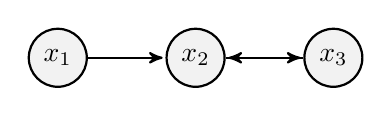
\begin{tikzpicture}
            \begin{scope}[->,>=stealth',shorten >=1pt,auto,node distance=1.75cm,thick, main node/.style={circle,fill=gray!10,draw}]
            \node[main node] (1) {$x_1$};
            \node[main node] (2) [right of=1] {$x_2$};
            \node[main node] (3) [right of=2] {$x_3$};
            \path[every node/.style={font=\sffamily\small}]
            (1) edge node[below] {} (2)
            (2) edge node [above] {} (3)
            (3) edge node [above] {} (2);
            %edge node[right] {} (5)
            %(4) edge node [above] {} (5)
            %(4) edge node [above] {} (5);
            \end{scope}
        \end{tikzpicture}  
    \end{center}  
    
    Let $x_j(t)$ be the number of particles residing at the $j$th lattice point at time $t$. Assume that $x_j$ satisfies the following rate equations.
    \begin{align*} 
        \frac{dx_1(t)}{dt} &= -kx_1 \\
        \frac{dx_2(t)}{dt} &= kx_1 + k(x_3 - x_2) \\
        \frac{dx_3(t)}{dt} &= k(x_2 - x_3) 
    \end{align*} % {{-2,1,0,1},{1,-3,1,1},{0,1,-2,1},{1,1,1,-3}}
    Assume $k > 0$ and $t \ge 0$. 
    \begin{parts} 
        \part Express the system of equations in the form $\vec x \, ' = A \vec x$. \vspace{2cm}
        \part The eigenvalues of $A$ are $0, -1, -2$.   Compute the eigenvectors of $A$. Show your work. 
        \newpage 
        \part (Question 1 continued) Use your results from parts (a) and (b) to determine the solution to the IVP $$\vec x \, ' = A \vec x, \quad \vec x(0) = \begin{pmatrix}1\\0\\0 \end{pmatrix}.$$
        Show your work. 
        \vspace{16cm}
        \part Use your results from part (c) to determine what $\vec x$ converges to as $t \to \infty$.
    \end{parts}


    % \newpage \Initials

    % \question[5] Solve the following initial value problem. Obtain an explicit expression for $y(t)$ Show your work. 
    % $$t^2y' - 6ty = 3t^3+14, \quad t \ge 0, \quad y(1) = 4$$

    

    
    
    
    \newpage \Initials
    \question[10] %2.5.11 verbatim 
    Consider the differential equation $\displaystyle \dydt = \frac12y(y-\frac12)^2$, where $y$ is a real function of $t$, and $t \ge 0$, and $k>0$. 
    \begin{parts}
        \part State the critical points of the differential equation.  \vspace{1cm} 
        \part Draw the phase line, and determine whether the critical points (if any) are stable, semi-stable, or unstable. Show your work. 
        \vspace{6cm}
        \part Determine where $y$ is concave up and concave down for $y \ge 0$. Show your work. 
        \vspace{6cm}
        \part Using results from parts (a), (b), and (c) to sketch several solution curves in the $ty$-plane for $t \ge 0$. 
    \end{parts}
    
    



    \newpage \Initials
    \question[8] Consider the linear system. $$\vec x \, ' = A \vec x, \quad A = \begin{pmatrix} 8&-2\\2&4 \end{pmatrix}, \quad \vec x = \vec x(t) = \begin{pmatrix} x_1(t) \\ x_2(t) \end{pmatrix}$$
    \begin{parts}
        \part[4] Determine the eigenvalues and eigenvectors of $A$. Show your work. \vspace{8cm}
        \part[4] Express the general solution of the system in terms of real valued functions.
        \vspace{8cm} 
        % % \newpage 
        % \part[3] Sketch the phase portrait of the system. Please include the eigenspaces in your sketch, indicate the direction of motion of your solution curves and eigenspaces, and do not forget to label your axes.      
        % \vspace{4cm} 
    \end{parts}



    \newpage \Initials
    \question[10] Solve the IVP using the method of undetermined coefficients.
    $$y''+20y'=324te^{-2t}, \quad y(0)=0, \quad y'(0) = 1$$
    
    








    \newpage \Initials

    \question[3] % ad hoc
    Consider the homogeneous system $\displaystyle \vec x \, ' = A \vec x = \spalignmat{\alpha, -1;1, \alpha}\vec x, \ \alpha \in \mathbb R$. 
    \begin{parts}
        \part Determine the eigenvalues of $A$ in terms of $\alpha$. 
        \vspace{5cm} 
        
        \part Identify the values of $\alpha$ (if any) where the qualitative nature of phase portrait for system changes. 
        \vspace{4cm} 
        
        \part For one value of $\alpha$ that you listed in part (b), sketch the phase portrait for a value of $\alpha$ that is less than the value that you identified, and one phase portrait for a value of $\alpha$ that is greater than the value you identified. Indicate the value of $\alpha$ that you selected and do not forget to label your axes. Indicate the direction of motion in your phase plane trajectories. 
    \end{parts}
    
    
    
    \newpage \Initials
    \question[1] One point will be allocated for presentation, neatness, and organization. Please ensure that
    \begin{enumerate}
        % \item your scan is under 5 MB in file size
        \item your work is legible in the scan
        \item your name or initials are at the top of every page
        \item questions are answered in the order in which they were given
        \item during the upload process you have indicated which pages correspond to which question, and made sure that none of your pages are upside down or sideways (you can also change the orientation of the pages when you upload in Gradescope)
    \end{enumerate}
    Ensuring that these criteria are met helps ensure that your exam is graded efficiently and accurately. 
        
    Please sign and date the following GT Honor Code statement. \\ 
    
    \vspace{6pt}
    \textbf{Georgia Tech Honor Code}\\
    \GTHonorCode
    
    \begin{center}
        \def\arraystretch{0.35}%  1 is the default, change whatever you need
        \begin{tabular}{ b{8cm} b{8cm} }
        \vspace{.5cm} \underline{\hspace{7cm}} & \vspace{.5cm} \underline{\hspace{4.5cm}}  \tabularnewline
        \vspace{6pt} signature & \vspace{6pt} date    
        \end{tabular}
    \end{center}
\end{questions}

\end{document}











    % \newpage \Initials
    % \question[10] Consider the initial value problem. 
    % $$
    % \vec x \, ' = A\vec x, \quad A = \begin{pmatrix} 5&-1&2\\2&2&2\\2&-1&5\end{pmatrix}, \quad \vec x(0) = \begin{pmatrix} 2\\5\\5 \end{pmatrix}, \quad \vec x = \vec x(t)
    % $$
    % \begin{parts} 
    %     \part Determine the eigenvectors of $A$ and use them to write down the general solution to the system of differential equations. You may use that the eigenvalues of $A$ are $\lambda_1=6$ and $\lambda_2 = 3$, and one of the eigenvalues has a multiplicity of two. \textit{Show your work when computing the eigenvectors: it is ok to check your work with software, but you should show that you can compute eigenvectors by hand. }
    %     \newpage 
    %     \part Use your result from the previous part to solve the IVP. 
    % \end{parts}